%  LaTeX support: latex@mdpi.com 
%  For support, please attach all files needed for compiling as well as the log file, and specify your operating system, LaTeX version, and LaTeX editor.
%=================================================================
\documentclass[journal,article,submit,pdftex,moreauthors]{Definitions/mdpi} 

%--------------------
% Class Options:
%--------------------
%----------
% journal
%----------
% Choose between the following MDPI journals:
% acoustics, actuators, addictions, admsci, adolescents, aerobiology, aerospace, agriculture, agriengineering, agrochemicals, agronomy, ai, air, algorithms, allergies, alloys, analytica, analytics, anatomia, animals, antibiotics, antibodies, antioxidants, applbiosci, appliedchem, appliedmath, applmech, applmicrobiol, applnano, applsci, aquacj, architecture, arm, arthropoda, arts, asc, asi, astronomy, atmosphere, atoms, audiolres, automation, axioms, bacteria, batteries, bdcc, behavsci, beverages, biochem, bioengineering, biologics, biology, biomass, biomechanics, biomed, biomedicines, biomedinformatics, biomimetics, biomolecules, biophysica, biosensors, biotech, birds, bloods, blsf, brainsci, breath, buildings, businesses, cancers, carbon, cardiogenetics, catalysts, cells, ceramics, challenges, chemengineering, chemistry, chemosensors, chemproc, children, chips, cimb, civileng, cleantechnol, climate, clinpract, clockssleep, cmd, coasts, coatings, colloids, colorants, commodities, compounds, computation, computers, condensedmatter, conservation, constrmater, cosmetics, covid, crops, cryptography, crystals, csmf, ctn, curroncol, cyber, dairy, data, ddc, dentistry, dermato, dermatopathology, designs, devices, diabetology, diagnostics, dietetics, digital, disabilities, diseases, diversity, dna, drones, dynamics, earth, ebj, ecologies, econometrics, economies, education, ejihpe, electricity, electrochem, electronicmat, electronics, encyclopedia, endocrines, energies, eng, engproc, entomology, entropy, environments, environsciproc, epidemiologia, epigenomes, est, fermentation, fibers, fintech, fire, fishes, fluids, foods, forecasting, forensicsci, forests, foundations, fractalfract, fuels, future, futureinternet, futurepharmacol, futurephys, futuretransp, galaxies, games, gases, gastroent, gastrointestdisord, gels, genealogy, genes, geographies, geohazards, geomatics, geosciences, geotechnics, geriatrics, grasses, gucdd, hazardousmatters, healthcare, hearts, hemato, hematolrep, heritage, higheredu, highthroughput, histories, horticulturae, hospitals, humanities, humans, hydrobiology, hydrogen, hydrology, hygiene, idr, ijerph, ijfs, ijgi, ijms, ijns, ijpb, ijtm, ijtpp, ime, immuno, informatics, information, infrastructures, inorganics, insects, instruments, inventions, iot, j, jal, jcdd, jcm, jcp, jcs, jcto, jdb, jeta, jfb, jfmk, jimaging, jintelligence, jlpea, jmmp, jmp, jmse, jne, jnt, jof, joitmc, jor, journalmedia, jox, jpm, jrfm, jsan, jtaer, jvd, jzbg, kidneydial, kinasesphosphatases, knowledge, land, languages, laws, life, liquids, literature, livers, logics, logistics, lubricants, lymphatics, machines, macromol, magnetism, magnetochemistry, make, marinedrugs, materials, materproc, mathematics, mca, measurements, medicina, medicines, medsci, membranes, merits, metabolites, metals, meteorology, methane, metrology, micro, microarrays, microbiolres, micromachines, microorganisms, microplastics, minerals, mining, modelling, molbank, molecules, mps, msf, mti, muscles, nanoenergyadv, nanomanufacturing,\gdef\@continuouspages{yes}} nanomaterials, ncrna, ndt, network, neuroglia, neurolint, neurosci, nitrogen, notspecified, %%nri, nursrep, nutraceuticals, nutrients, obesities, oceans, ohbm, onco, %oncopathology, optics, oral, organics, organoids, osteology, oxygen, parasites, parasitologia, particles, pathogens, pathophysiology, pediatrrep, pharmaceuticals, pharmaceutics, pharmacoepidemiology,\gdef\@ISSN{2813-0618}\gdef\@continuous pharmacy, philosophies, photochem, photonics, phycology, physchem, physics, physiologia, plants, plasma, platforms, pollutants, polymers, polysaccharides, poultry, powders, preprints, proceedings, processes, prosthesis, proteomes, psf, psych, psychiatryint, psychoactives, publications, quantumrep, quaternary, qubs, radiation, reactions, receptors, recycling, regeneration, religions, remotesensing, reports, reprodmed, resources, rheumato, risks, robotics, ruminants, safety, sci, scipharm, sclerosis, seeds, sensors, separations, sexes, signals, sinusitis, skins, smartcities, sna, societies, socsci, software, soilsystems, solar, solids, spectroscj, sports, standards, stats, std, stresses, surfaces, surgeries, suschem, sustainability, symmetry, synbio, systems, targets, taxonomy, technologies, telecom, test, textiles, thalassrep, thermo, tomography, tourismhosp, toxics, toxins, transplantology, transportation, traumacare, traumas, tropicalmed, universe, urbansci, uro, vaccines, vehicles, venereology, vetsci, vibration, virtualworlds, viruses, vision, waste, water, wem, wevj, wind, women, world, youth, zoonoticdis 
% For posting an early version of this manuscript as a preprint, you may use "preprints" as the journal. Changing "submit" to "accept" before posting will remove line numbers.

%---------
% article
%---------
% The default type of manuscript is "article", but can be replaced by: 
% abstract, addendum, article, book, bookreview, briefreport, casereport, comment, commentary, communication, conferenceproceedings, correction, conferencereport, entry, expressionofconcern, extendedabstract, datadescriptor, editorial, essay, erratum, hypothesis, interestingimage, obituary, opinion, projectreport, reply, retraction, review, perspective, protocol, shortnote, studyprotocol, systematicreview, supfile, technicalnote, viewpoint, guidelines, registeredreport, tutorial
% supfile = supplementary materials

%----------
% submit
%----------
% The class option "submit" will be changed to "accept" by the Editorial Office when the paper is accepted. This will only make changes to the frontpage (e.g., the logo of the journal will get visible), the headings, and the copyright information. Also, line numbering will be removed. Journal info and pagination for accepted papers will also be assigned by the Editorial Office.

%------------------
% moreauthors
%------------------
% If there is only one author the class option oneauthor should be used. Otherwise use the class option moreauthors.

%---------
% pdftex
%---------
% The option pdftex is for use with pdfLaTeX. Remove "pdftex" for (1) compiling with LaTeX & dvi2pdf (if eps figures are used) or for (2) compiling with XeLaTeX.

%=================================================================
% MDPI internal commands - do not modify
\firstpage{1} 
\makeatletter 
\setcounter{page}{\@firstpage} 
\makeatother
\pubvolume{1}
\issuenum{1}
\articlenumber{0}
\pubyear{2024}
\copyrightyear{2024}
%\externaleditor{Academic Editor: Firstname Lastname}
\datereceived{ } 
\daterevised{ } % Comment out if no revised date
\dateaccepted{ } 
\datepublished{ } 
%\datecorrected{} % For corrected papers: "Corrected: XXX" date in the original paper.
%\dateretracted{} % For corrected papers: "Retracted: XXX" date in the original paper.
\hreflink{https://doi.org/} % If needed use \linebreak
%\doinum{}
%\pdfoutput=1 % Uncommented for upload to arXiv.org
%\CorrStatement{yes}  % For updates


%=================================================================
% Add packages and commands here. The following packages are loaded in our class file: fontenc, inputenc, calc, indentfirst, fancyhdr, graphicx, epstopdf, lastpage, ifthen, float, amsmath, amssymb, lineno, setspace, enumitem, mathpazo, booktabs, titlesec, etoolbox, tabto, xcolor, colortbl, soul, multirow, microtype, tikz, totcount, changepage, attrib, upgreek, array, tabularx, pbox, ragged2e, tocloft, marginnote, marginfix, enotez, amsthm, natbib, hyperref, cleveref, scrextend, url, geometry, newfloat, caption, draftwatermark, seqsplit
% cleveref: load \crefname definitions after \begin{document}

%=================================================================
% Please use the following mathematics environments: Theorem, Lemma, Corollary, Proposition, Characterization, Property, Problem, Example, ExamplesandDefinitions, Hypothesis, Remark, Definition, Notation, Assumption
%% For proofs, please use the proof environment (the amsthm package is loaded by the MDPI class).

%=================================================================
% Full title of the paper (Capitalized)
\Title{A machine learning model for forecast procurement of secondary reserve capacity in power systems with significant vRES penetrations}

% MDPI internal command: Title for citation in the left column
\TitleCitation{Title}

% Author Orchid ID: enter ID or remove command
\newcommand{\orcidauthorA}{0009-0007-5995-8060} % Add \orcidA{} behind the author's name
%\newcommand{\orcidauthorB}{0000-0000-0000-000X} % Add \orcidB{} behind the author's name

% Authors, for the paper (add full first names)
\Author{João Passagem Santos \orcidA{}, Hugo Algarvio and Ana Estanqueiro}

%\longauthorlist{yes}

% MDPI internal command: Authors, for metadata in PDF
\AuthorNames{João Passagem Santos, Hugo Algarvio and Ana Estanqueiro}

% MDPI internal command: Authors, for citation in the left column
\AuthorCitation{Passagem Santos, J.; Algarvio, H.; Estanqueiro, A.}
% If this is a Chicago style journal: Lastname, Firstname, Firstname Lastname, and Firstname Lastname.

% Affiliations / Addresses (Add [1] after \address if there is only one affiliation.)
\address{%
$^{1}$ \quad Affiliation 1; e-mail@e-mail.com\\
$^{2}$ \quad Affiliation 2; e-mail@e-mail.com}

% Contact information of the corresponding author
% \corres{Correspondence: e-mail@e-mail.com; Tel.: (optional; include country code; if there are multiple corresponding authors, add author initials) +xx-xxxx-xxx-xxxx (F.L.)}

% % Current address and/or shared authorship
% \firstnote{Current address: Affiliation.}  % Current address should not be the same as any items in the Affiliation section.
% \secondnote{These authors contributed equally to this work.}
% The commands \thirdnote{} till \eighthnote{} are available for further notes

%\simplesumm{} % Simple summary

%\conference{} % An extended version of a conference paper

% Abstract (Do not insert blank lines, i.e. \\) 
\abstract{The growing investment in variable renewable energy sources is changing how electricity markets operate. Players rely on forecasts to participate in markets closing between 1 and 37 hours ahead of real-time operation.  Usually,  transmission system operators (TSOs) use a symmetrical procurement of up and down secondary power reserves based on the expected demand. This work uses machine learning techniques that dynamically computes it using the day-ahead programmed and expected dispatches of variable renewables, demand, and other technologies. The study uses operational open data from the Spanish TSO from 2014 to 2023 for training. Benchmark and test data are from the period of 2019 to 2022. The proposed methodology improves the usage of the up and down secondary reserved power by almost 47\% and 42\%, respectively.}

% Keywords
\keyword{reserve systems; energy markets; neural networks; forecast} 

% The fields PACS, MSC, and JEL may be left empty or commented out if not applicable
%\PACS{J0101}
%\MSC{}
%\JEL{}

%%%%%%%%%%%%%%%%%%%%%%%%%%%%%%%%%%%%%%%%%%
% Only for the journal Diversity
%\LSID{\url{http://}}

%%%%%%%%%%%%%%%%%%%%%%%%%%%%%%%%%%%%%%%%%%
% Only for the journal Applied Sciences
%\featuredapplication{Authors are encouraged to provide a concise description of the specific application or a potential application of the work. This section is not mandatory.}
%%%%%%%%%%%%%%%%%%%%%%%%%%%%%%%%%%%%%%%%%%

%%%%%%%%%%%%%%%%%%%%%%%%%%%%%%%%%%%%%%%%%%
% Only for the journal Data
%\dataset{DOI number or link to the deposited data set if the data set is published separately. If the data set shall be published as a supplement to this paper, this field will be filled by the journal editors. In this case, please submit the data set as a supplement.}
%\datasetlicense{License under which the data set is made available (CC0, CC-BY, CC-BY-SA, CC-BY-NC, etc.)}

%%%%%%%%%%%%%%%%%%%%%%%%%%%%%%%%%%%%%%%%%%
% Only for the journal Toxins
%\keycontribution{The breakthroughs or highlights of the manuscript. Authors can write one or two sentences to describe the most important part of the paper.}

%%%%%%%%%%%%%%%%%%%%%%%%%%%%%%%%%%%%%%%%%%
% Only for the journal Encyclopedia
%\encyclopediadef{For entry manuscripts only: please provide a brief overview of the entry title instead of an abstract.}

%%%%%%%%%%%%%%%%%%%%%%%%%%%%%%%%%%%%%%%%%%
% Only for the journal Advances in Respiratory Medicine and Smart Cities
%\addhighlights{yes}
%\renewcommand{\addhighlights}{%

%\noindent This is an obligatory section in “Advances in Respiratory Medicine'' and ``Smart Cities”, whose goal is to increase the discoverability and readability of the article via search engines and other scholars. Highlights should not be a copy of the abstract, but a simple text allowing the reader to quickly and simplified find out what the article is about and what can be cited from it. Each of these parts should be devoted up to 2~bullet points.\vspace{3pt}\\
%\textbf{What are the main findings?}
% \begin{itemize}[labelsep=2.5mm,topsep=-3pt]
% \item First bullet.
% \item Second bullet.
% \end{itemize}\vspace{3pt}
%\textbf{What is the implication of the main finding?}
% \begin{itemize}[labelsep=2.5mm,topsep=-3pt]
% \item First bullet.
% \item Second bullet.
% \end{itemize}
%}

%%%%%%%%%%%%%%%%%%%%%%%%%%%%%%%%%%%%%%%%%%
\begin{document}

%%%%%%%%%%%%%%%%%%%%%%%%%%%%%%%%%%%%%%%%%%
% \setcounter{section}{-1} %% Remove this when starting to work on the template.
% \section{How to Use this Template}

% The template details the sections that can be used in a manuscript. Note that the order and names of article sections may differ from the requirements of the journal (e.g., the positioning of the Materials and Methods section). Please check the instructions on the authors' page of the journal to verify the correct order and names. For any questions, please contact the editorial office of the journal or support@mdpi.com. For LaTeX-related questions please contact latex@mdpi.com.%\endnote{This is an endnote.} % To use endnotes, please un-comment \printendnotes below (before References). Only journal Laws uses \footnote.

% % The order of the section titles is different for some journals. Please refer to the "Instructions for Authors” on the journal homepage.

% \section{Introduction}

% The introduction should briefly place the study in a broad context and highlight why it is important. It should define the purpose of the work and its significance. The current state of the research field should be reviewed carefully and key publications cited. Please highlight controversial and diverging hypotheses when necessary. Finally, briefly mention the main aim of the work and highlight the principal conclusions. As far as possible, please keep the introduction comprehensible to scientists outside your particular field of research. Citing a journal paper \cite{ref-journal}. Now citing a book reference \cite{ref-book1,ref-book2} or other reference types \cite{ref-unpublish,ref-communication,ref-proceeding}. Please use the command \citep{ref-thesis,ref-url} for the following MDPI journals, which use author--date citation: Administrative Sciences, Arts, Econometrics, Economies, Genealogy, Humanities, IJFS, Journal of Intelligence, Journalism and Media, JRFM, Languages, Laws, Religions, Risks, Social Sciences, Literature.

%%%%%%%%%%%%%%%%%%%%%%%%%%%%%%%%%%%%%%%%%%
%%%%%%%%%%%%%%%%%%%%%%%%%%%%%%%%%%%%%%%%%%
%%%%%%%%%%%%%%%%%%%%%%%%%%%%%%%%%%%%%%%%%%

\section{Introduction}


The European Union's energy and climate goals for 2030 and 2050 emphasize the transition to a carbon-neutral energy system, driven by the large-scale integration of variable renewable energy sources (vRES), such as wind and solar photovoltaic (PV) technologies. While vRES are critical for achieving sustainability targets, such as SDG 7 (Affordable and Clean Energy) and SDG 13 (Climate Action), their stochastic and intermittent nature poses significant challenges to power system operations, particularly in balancing energy supply and demand efficiently. \par
The increasing penetration of vRES introduces greater uncertainty into energy markets, particularly in day-ahead forecasts, which are essential for the allocation of secondary reserves. These reserves, procured to address real-time imbalances between generation and consumption, often suffer from inefficient allocation methodologies. Day-ahead predictions frequently diverge from real-time conditions, leading to both over-allocation and under-allocation of reserves. This inefficiency not only results in higher operational costs but also compromises the optimal utilization of resources, thereby undermining the economic and energy efficiency of the system.\par
This paper focuses on enhancing the accuracy of day-ahead forecasts for secondary reserve allocation, addressing the inefficiencies caused by vRES uncertainty. By leveraging machine learning techniques, this work develops predictive models that incorporate historical data on vRES generation, demand patterns, and system behavior. The objective is to dynamically adjust reserve allocations, ensuring that grid stability is maintained while minimizing excess reserve procurement.\par
The study evaluates the impact of dynamic reserve allocation on reserve markets, exploring its potential to improve market efficiency and reduce costs. By accurately predicting reserve needs, the proposed approach aims to reduce the uncertainties associated with vRES and contribute to a more robust and cost-effective energy system.\par
The remainder of this paper is structured as follows. Section II provides an overview of wholesale energy markets and reserve systems, highlighting existing inefficiencies. Section III outlines the proposed methodology for dynamic reserve allocation using machine learning techniques. Section IV presents case studies and evaluates the performance of the developed models. Finally, Section V summarizes the findings and discusses the implications for future energy systems.\par

\par
\par

The growing integration of variable renewable energy sources (vRES), such as wind and solar photovoltaic (PV) technologies, is transforming electricity systems across Europe. While vRES play a crucial role in achieving carbon neutrality goals and addressing climate targets set for 2030 and 2050, their intermittent and stochastic nature introduces significant operational challenges. These challenges are particularly evident in the accurate forecasting of energy generation and consumption, which is critical for efficient reserve management.\par
Transmission System Operators (TSOs) rely on day-ahead markets to procure secondary reserves, balancing supply and demand in real time. However, the volatility of vRES production often leads to discrepancies between forecasted and actual conditions, resulting in over-allocation or under-allocation of reserves. Inaccurate allocation increases operational costs, reduces system efficiency, and hampers the optimal use of resources. Addressing this issue is essential for improving grid stability and ensuring the cost-effectiveness of energy markets.\par
Dynamic allocation of secondary reserves has emerged as a promising solution to mitigate these inefficiencies, particularly when supported by advanced predictive tools. Recent studies have demonstrated the potential of machine learning techniques to enhance forecast accuracy, enabling better alignment of reserve procurement with real-time system needs. By analyzing historical operational data and identifying patterns in vRES generation, demand, and system behavior, machine learning models can significantly reduce forecasting errors and improve the efficiency of reserve allocation.\par
This paper proposes a machine learning-based methodology for the dynamic procurement of secondary reserves, using historical and operational data from the Spanish electricity market as a case study. The approach aims to optimize reserve allocation, minimize inefficiencies caused by vRES variability, and improve the overall management of balancing services. The results demonstrate the potential of machine learning techniques to enhance system reliability and reduce unnecessary reserve costs in markets with high renewable penetration.\par
The remainder of this paper is structured as follows. Section II reviews the literature on electricity markets and reserve systems. Section III introduces the proposed dynamic allocation methodology. Section IV presents the case study and evaluates the results. Finally, Section V concludes with a discussion on the implications and potential for future work.\par
\label{introduction}

\section{Literature review}
The increasing integration of \gls{vRES} in power systems has created significant challenges for electricity markets and ancillary services. Traditionally, \gls{TSO} rely on symmetric allocation of upward and downward reserves based on deterministic forecasts of demand. However, with \gls{vRES} like wind and solar introducing substantial variability and unpredictability, these conventional methods have proven inefficient in addressing the real-time balancing needs of modern power grids.\par
Numerous studies highlight the limitations of static reserve procurement methods under high vRES penetration. The \gls{ENTSO-E} framework \cite{handbook2009policy} outlines standardized methodologies for reserve sizing, which are \gls{FCR}, \gls{aFRR} and \gls{mFRR}, but these often fail to adapt dynamically to changing system conditions. In Portugal, for example, the secondary reserve allocation formula used by the \gls{TSO} employs a fixed ratio applied to expected demand, resulting in excessive allocation and energy waste %[2]
. Similar inefficiencies are observed in the Spanish market, where reserve procurement lacks symmetry and adaptability to \gls{vRES} production.\par %[3]
%
The majority of the literature focuses on using historical data to compute the procurement of secondary reserves \cite{Knorr:19,Frade2019_market,Papavasiliou:21}
%
Operational methodologies are needed to be used by TSOs.

Dynamic procurement of secondary reserves has been proposed as a solution to address these inefficiencies, with an improvement in 13\% and 8\% for up and down secondary capacities by 2022 \cite{Algarvio2024}. By incorporating real-time or near real-time forecasts of demand and renewable generation, dynamic methodologies aim to optimize reserve allocation, reducing both operational costs and resource wastage.
%
Furthermore, five different mechanisms for procuring secondary power in Spain were analyzed for the Spanish power system by 2030, with renewable penetrations higher than 70\% \cite{Algarvio:24}. The dynamic procurement methodology proposed in this study enables cost reductions for Spanish secondary power by 27\% when using block bids and 34\% when using flexible bids. These results highlight the increasing importance of dynamic reserve procurements with the rising uncertainty of higher penetrations of \gls{vRES}.  
%
Machine learning techniques have emerged as a powerful tool to support this transition. Studies such as \cite{DeVos2019} and \cite{Kruse2022} demonstrate the potential of predictive models to estimate reserve needs with greater accuracy, leading to significant reductions in over-procurement. 
De Vos et \textit{al.} proposed a machine learning approach to estimate imbalance uncertainty, with the goal of adjusting the size of Belgium's operating reserves from an annual to a daily basis, resulting in a 5\% reduction \cite{DeVos2019}. Kruse, Sch\"{a}fer, and Witthaut introduced an ex-post machine learning method to determine the appropriate size for secondary reserves. They identified key variables that most accurately estimate errors, which are essential for detecting when secondary control is activated. Additionally, to enhance the efficiency of cross-border capacity allocation in balancing service exchanges, legislation recommended coupling balancing mechanisms, as demonstrated in the Nordpool market \cite{Frade:19c,Khodadadi:20}.\par
The literature also underscores the importance of enhancing forecast accuracy for \gls{vRES} generation and consumption patterns. Traditional statistical models, including ARMA and ARIMA, have been widely used for time series forecasting. However, recent advancements in machine learning, such as \gls{LSTM} networks and \gls{CNN}, have shown superior performance in capturing the nonlinear and temporal characteristics of renewable energy data \cite{Benti2023}. These models can adapt to complex patterns and improve prediction accuracy, enabling more efficient management of reserves.\par
In summary, the literature identifies three key areas of focus: the inefficiency of static reserve allocation methods, the potential of machine learning to improve forecasting accuracy, and the need for market design adaptations to support dynamic reserve procurement. This paper builds upon these insights by applying machine learning techniques to optimize secondary reserve allocation in the Spanish electricity market, addressing both forecast uncertainty and market inefficiencies.\par
\label{literary_review}

\section{Electricity Markets and Ancillary Services}
The operation of modern electricity systems relies heavily on well-structured markets to ensure the balance between generation and consumption. These markets encompass wholesale electricity markets, where energy is traded, and ancillary services markets, which guarantee the system's stability and reliability. The integration of \gls{vRES} has added complexity to these operations, requiring more dynamic approaches to market design and reserve allocation.\par

% \paragraph{Mercado de Serviços de Sistema \label{se:servicos_sistema_mibel}}
% \text{ }  \par
% Por fim, o mercado de serviços de sistema desempenha um papel crítico na manutenção do equilíbrio entre a produção e o consumo de energia elétrica em tempo real. Este mercado é responsável por garantir que a rede elétrica opere de forma segura e estável, ativando reservas e ajustando a produção conforme necessário para responder a variações inesperadas na procura ou na oferta. O mercado de serviços de sistema engloba uma série de mecanismos, incluindo a ativação de reservas de frequência e o despacho de unidades geradoras flexíveis, que são essenciais para a gestão da estabilidade da rede. A participação neste mercado é muitas vezes obrigatória para certos tipos de geradores, especialmente aqueles que possuem a capacidade de resposta rápida, como hidroelétricas e centrais térmicas.\par
% Os mercados de serviços de sistema, português e espanhol, são geridos independentemente, onde o \gls{GGS} é o operador do mercado no respectivo país, sendo a \gls{REN} em Portugal e a \gls{REE} em Espanha.\par
% \bigskip
% \bigskip
% Sumariamente, o \gls{MIBEL} é um mercado complexo e multifacetado que oferece uma ampla gama de formatos de negociação para atender às diversas necessidades dos agentes de mercado. Desde a negociação em tempo real no mercado \textit{spot} até compromissos de longo prazo no mercado de contratação a prazo e acordos personalizados no mercado bilateral, o \gls{MIBEL} proporciona um ambiente robusto para a transação de eletricidade, promovendo a eficiência, a flexibilidade e a segurança do fornecimento de energia na Península Ibérica.\cite{Rassid2017}\par

\subsection{Wholesale Electricity Markets}

Wholesale electricity markets facilitate the trading of electricity between generators, suppliers, and other market participants. These markets are typically divided into three main categories: \gls{DAM}, \gls{IDM}, and real-time balancing markets. In the \gls{DAM}, participants submit bids for energy delivery 12 to 37 hours before real-time operation. The market-clearing process determines the energy schedules and market prices based on supply and demand equilibrium \cite{Algarvio:19b}. While the \gls{DAM} provides a foundation for energy trading, \gls{IDM} allow participants to make adjustments closer to real-time, responding to unforeseen changes in demand or \gls{vRES} generation.\par

Balancing markets, on the other hand, operate in near real-time to address deviations between scheduled and actual energy delivery. \gls{TSO}s procure balancing services to ensure system equilibrium, activating reserves as needed. This process is particularly critical in systems with high \gls{vRES} penetration, where forecasting errors can cause significant imbalances \cite{Algarvio:19a}.\par

\subsection{Ancillary Services and Reserve Requirements}

Ancillary services are essential for maintaining grid stability and ensuring a reliable power supply. They include services such as frequency control, voltage regulation, and operating reserves. Among these, frequency control reserves play a crucial role in balancing supply and demand in real-time. These reserves are divided into three main categories \cite{Algarvio:19a} as presented in Figure~\ref{fig:Ancillary_Services_response_scheme}:

\begin{itemize}
    \item	\gls{FCR}: Activated automatically within seconds to stabilize frequency deviations.
    \item	\gls{aFRR}: Restore frequency to nominal levels and release FCR for subsequent use.
    \item	\gls{mFRR}: Address longer-term imbalances through manual activation.
\end{itemize}

% \begin{figure}[H]
% 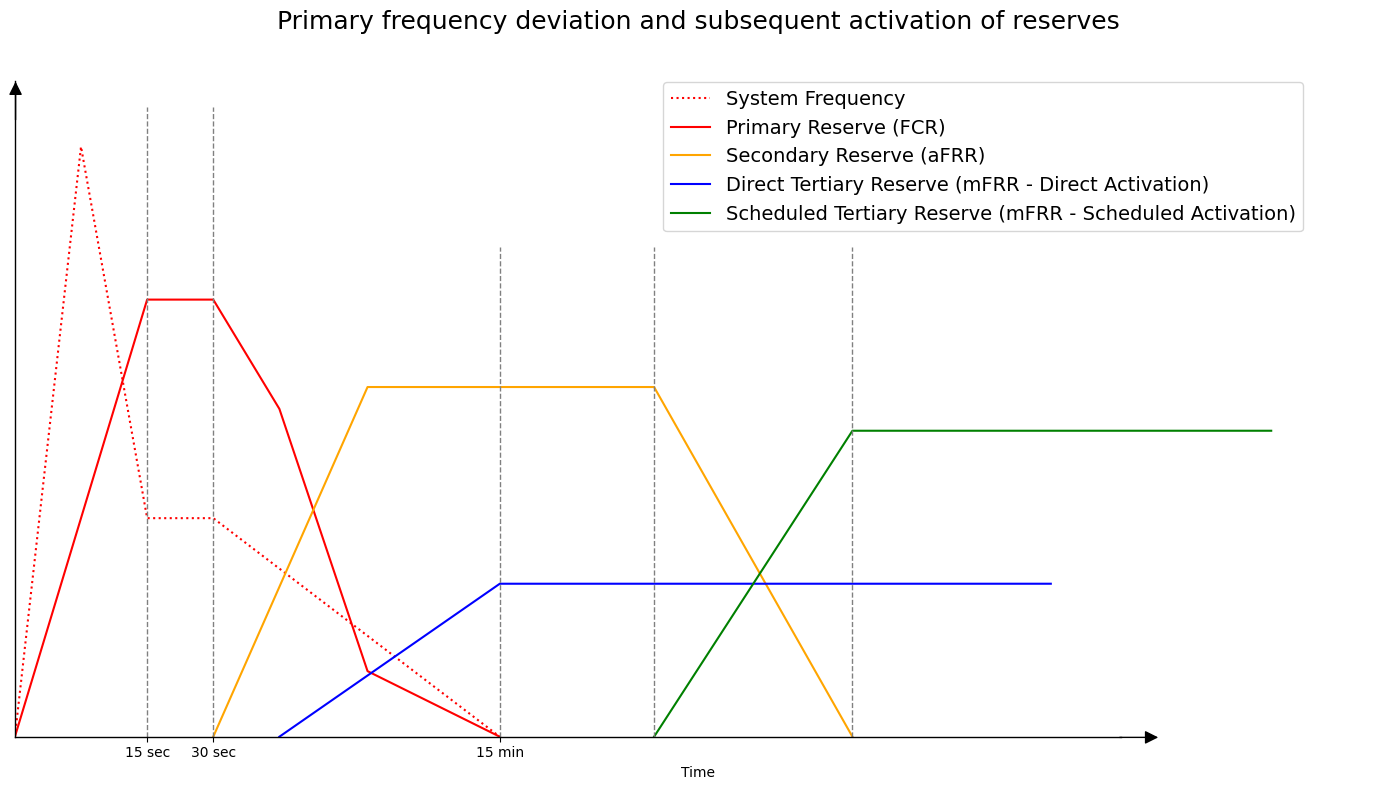
\includegraphics[width=10.5 cm]{plots/actiavtion_example_eng.png}
% \caption{Ancillary Services response scheme. Adapted from \cite{handbook2009policy}}
% \end{figure}   
% \unskip


\begin{figure}[H]
  \centering
  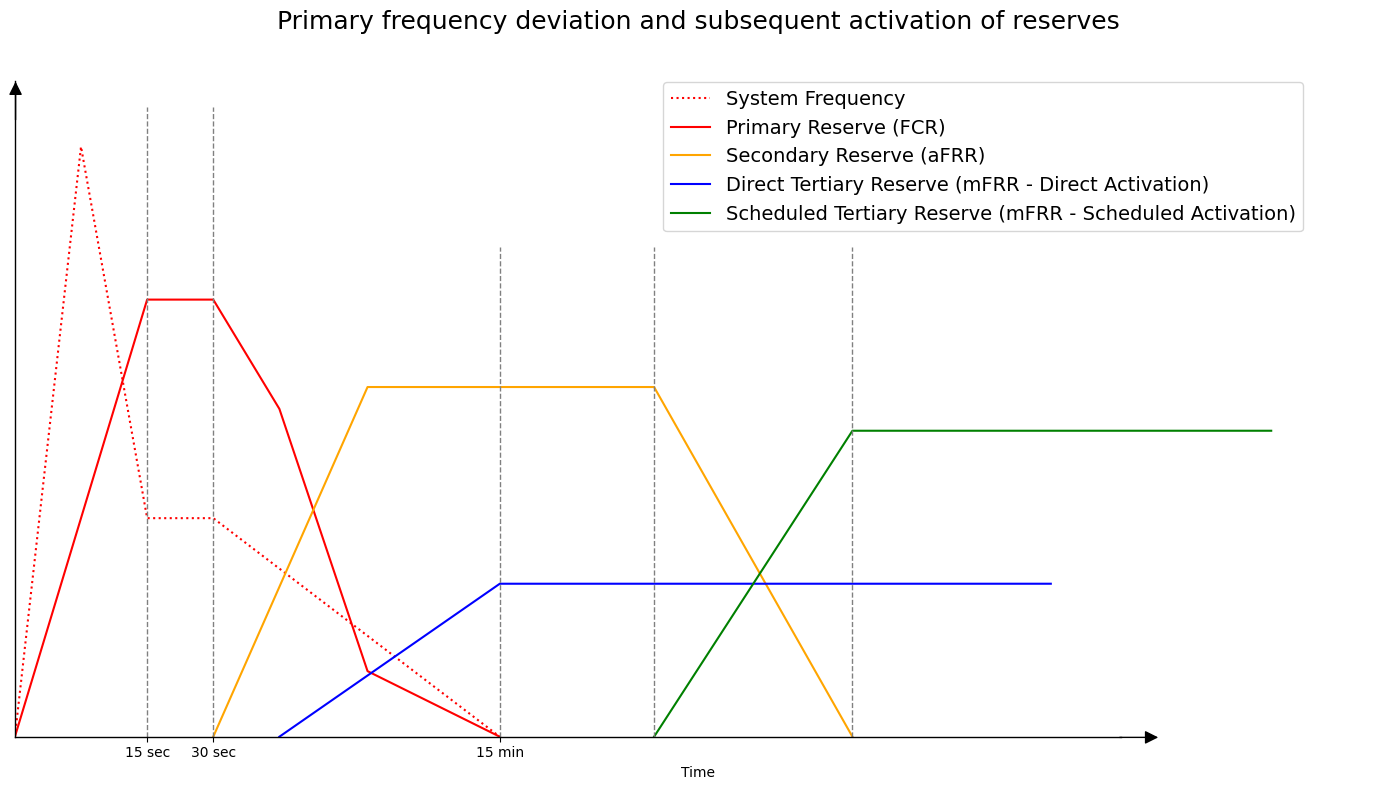
\includegraphics[width=\textwidth]{plots/actiavtion_example_eng.png}
  \caption{Ancillary Services response scheme. Adapted from \cite{handbook2009policy}}
  \label{fig:Ancillary_Services_response_scheme}
\end{figure}
\unskip



\subsection{Iberian Reserve Markets}

\gls{MIBEL} is the Iberian example of energy market integration across countries. Acting as a bond between Portuguese and Spanish electricity markets, \gls{OMIP} and \gls{OMIE}. This joint market consists of bilateral, derivatives, and spot markets.\par
Even though there is a joint market, each country's \gls{TSO}, \gls{REE} for Spain and \gls{REN} for Portugal, manages it's own ancillary services independently. 

\subsubsection{Static Reserve Procurement}
In Europe, the \gls{ENTSO-E} provides guidelines for the procurement and activation of these reserves. Traditionally, \gls{TSO}s acquire reserves symmetrically (equal upward and downward capacities), based on deterministic demand forecasts. However, this approach often leads to inefficiencies in systems with high \gls{vRES} variability.
%
For secundary reserve \gls{ENTSO-E} proposes:
\begin{linenomath}
\begin{equation}\label{eq:BRENTSOE} 
    R = \sqrt{a \times  L_{max} + b^{2}} - b 
\end{equation}
\end{linenomath}
where:

\begin{itemize}
  \item $R$: Secondary Control Reserve.
  \item $a$ and $b$: empiric coefficients, $a$=10MW and $b$=150MW .
  \item $L_{max}$: maximum anticipated consumer load.
\end{itemize}

The Spanish and Portuguese markets provide examples of differing reserve procurement methods. In Portugal, the \gls{TSO} employs a fixed ratio formula for secondary reserve sizing. Creating a symmetrical distribution for upward and downward bands, respectively $\frac{2}{3}$ and $\frac{1}{3}$ of the reserve band.\par
The given formula is based on \gls{ENTSO-E} equation \eqref{eq:BRENTSOE}, adding an hourly ratio $\rho$:

\begin{linenomath}
  \begin{equation}\label{eq:BRREN} 
    R = \rho \times \sqrt{a \times  L_{max} + b^{2}} - b 
  \end{equation}
  \end{linenomath}

The hourly ratio $\rho$ varies between 20\% (1.2) and 60\% (1.6), upscaling the the ENTSO-E suggestion for up regulation.

Conversely, the Spanish market lacks a standardized reserve procurement formula, relying instead on a more flexible procurement mechanism \cite{Frade2019_market}. Where the upward and downward bands distribution is not directly symmetric.
These differences highlight the need for market design improvements to better accommodate the variability of \gls{vRES}.




\label{markets_and_services}

\section{Dynamic procurement of secondary power}
The dynamic procurement of secondary reserves represents a significant step forward in addressing the inefficiencies inherent in traditional static allocation methods. Unlike static reserve procurement, which relies on fixed ratios or historical averages, dynamic approaches incorporate real-time forecasts and system conditions to adjust reserve requirements. This adaptability is particularly critical for modern electricity systems with high penetration of variable renewable energy sources (vRES), where forecasting uncertainty and rapid changes in generation output challenge grid stability.

Dynamic reserve procurement involves estimating upward and downward reserve needs based on the expected deviations between day-ahead scheduled generation and real-time demand. By leveraging advanced forecasting tools, such as machine learning models, it becomes possible to predict these deviations with greater accuracy, optimizing the allocation of secondary reserves. Historical data on vRES production, system demand, and grid imbalances serve as inputs to these models, allowing the identification of patterns and trends that inform reserve procurement decisions.

Machine learning techniques, including Long Short-Term Memory (LSTM) networks and other time-series forecasting models, have demonstrated significant potential for improving reserve predictions. These models can capture the nonlinear and temporal dependencies present in renewable energy data, outperforming traditional statistical methods such as ARIMA. By incorporating real-time weather forecasts, generation data, and demand profiles, dynamic approaches ensure that reserve procurement aligns more closely with actual system needs, reducing both over-procurement and under-procurement of reserves.

The dynamic approach also allows for asymmetrical procurement of upward and downward reserves, which is particularly relevant in systems with variable renewable generation. For instance, during periods of high solar generation, upward reserves may be less critical, whereas downward reserves become essential to accommodate excess production. Conversely, during low renewable output, upward reserves are prioritized to address potential generation shortfalls.

In summary, dynamic procurement of secondary reserves offers a more efficient and adaptive solution to balancing challenges in modern electricity systems. By leveraging machine learning techniques and real-time forecasts, this approach enhances reserve allocation, reduces operational costs, and
\label{procument}

\section{Case-study}
To evaluate the applicability of machine learning techniques for secondary reserve allocation, the study was conducted using the Spanish electricity market historical data from 2014 to 2024.

\subsection{Data Sources and Preprocessing}

The case study utilizes publicly available operational and historical data from the Spanish \gls{TSO}, \gls{REE} (please check the Data Availability Statement). The dataset includes the key variables presented in Table~\ref{esios_data}.

The data spans multiple years to account for seasonal variability and long-term trends in vRES generation and demand. Data preprocessing only handled missing values using interpolation methods, with IterativeImputer \cite{vanBuuren2011,Buck1960}, as presented in Figure~\ref{fig:misisng_data}.

To choose the temporal space of the models, temporal auto-correlations were checked in Table~\ref{temp_corr}.

\begin{figure}[H]
    \centering
    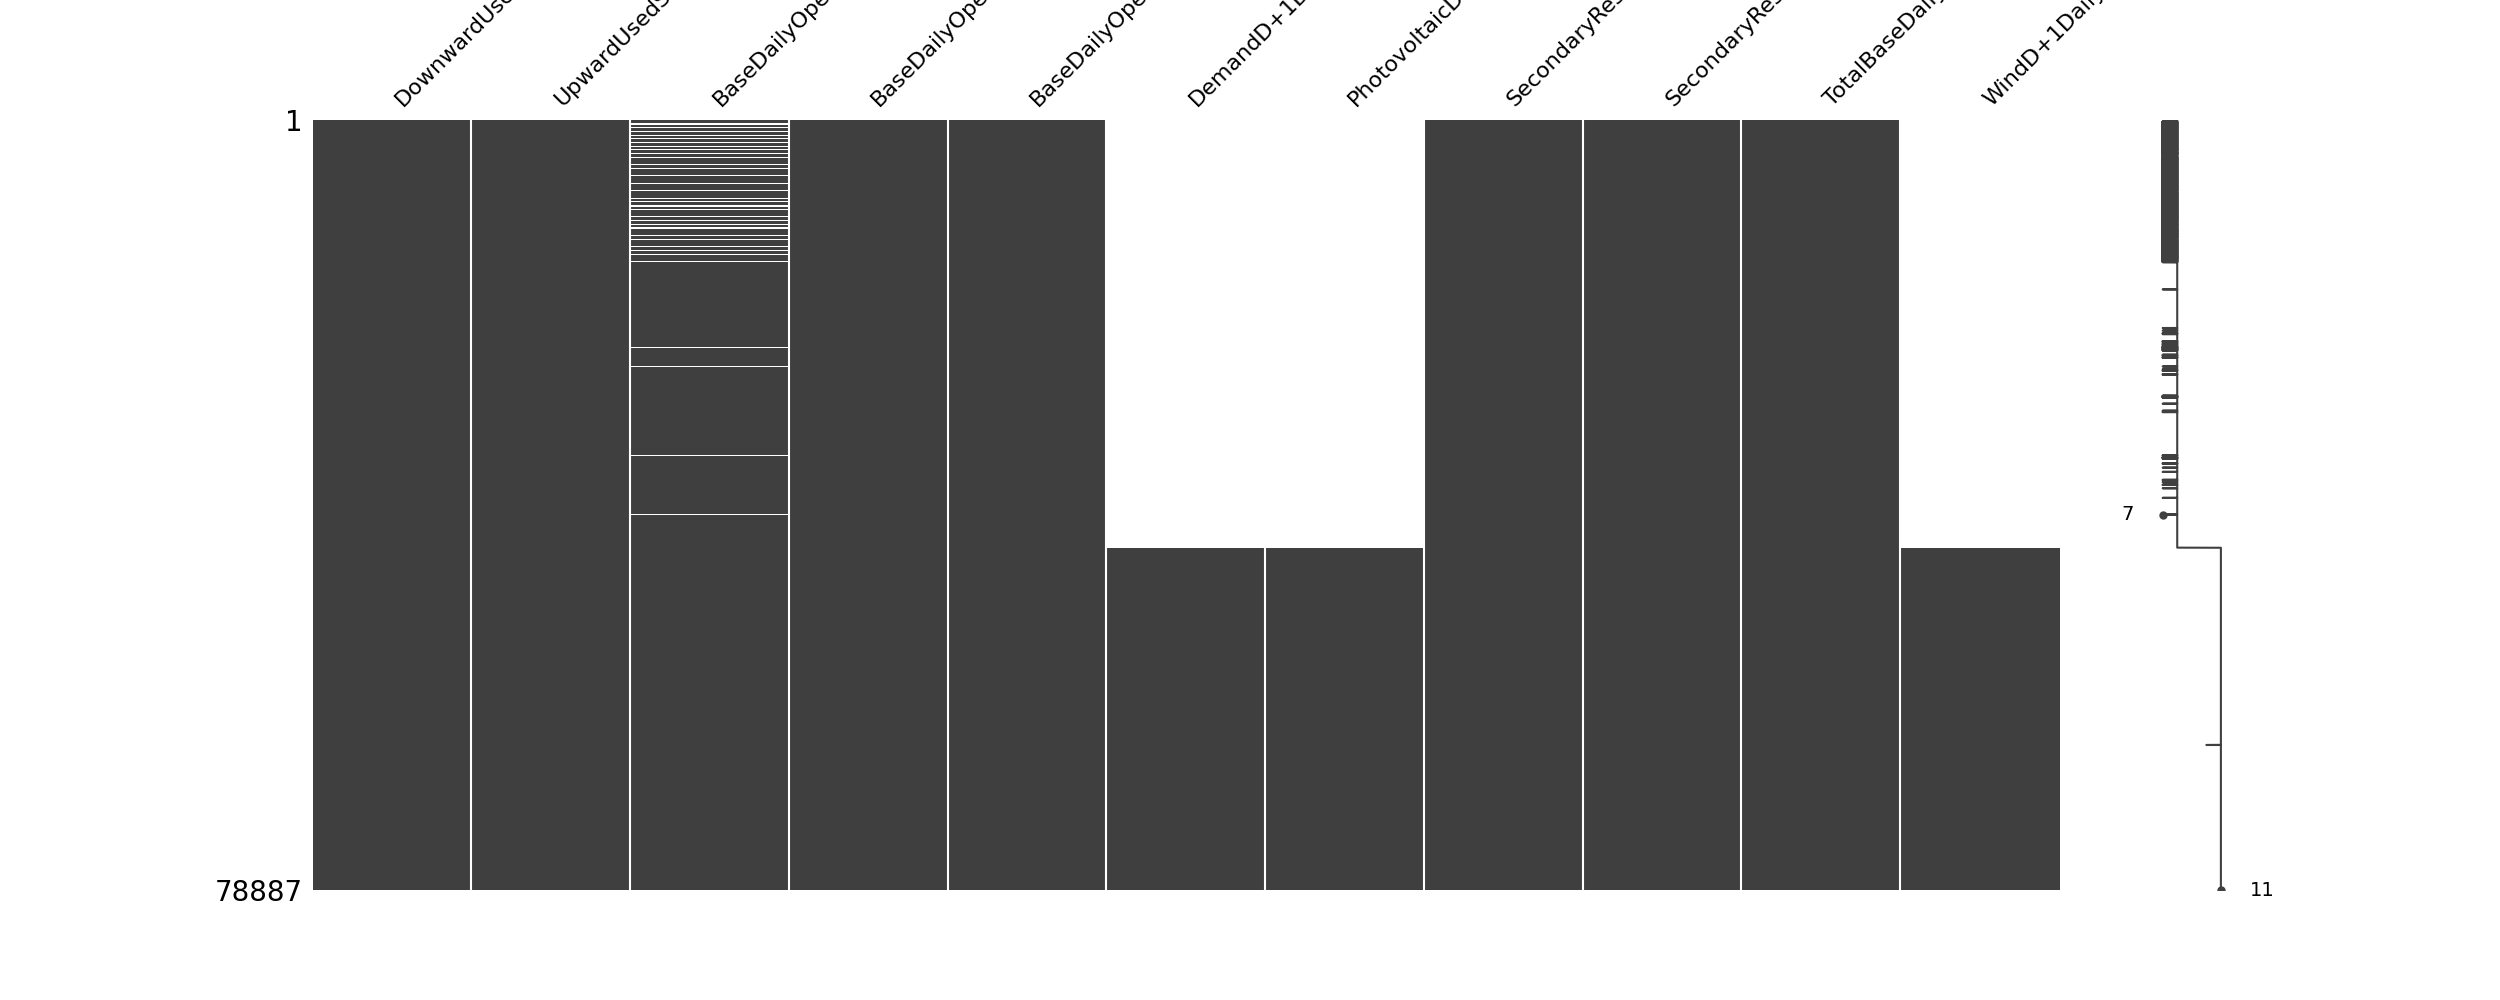
\includegraphics[width=\textwidth]{plots/missing_data.png}
    \caption{Missing Data.}
    \label{fig:misisng_data}
  \end{figure}

\begin{table}[H] 
\caption{This is a table caption. Tables should be placed in the main text near to the first time they are~cited.\label{tab1}}
\newcolumntype{C}{>{\centering\arraybackslash}X}
\begin{tabularx}{\textwidth}{CCCC}
\toprule
\textbf{ESIOS Code}	& \textbf{ESIOS Name} & \textbf{Variable}	& \textbf{Units}\\
\midrule
632 & Secondary Reserve Allocation AUpward     & Up Allocated & MW\\
633 & Secondary Reserve Allocation ADownward   & Down Allocated & MW\\
680 & Upward Used Secondary Reserve Energy  & Up Used & MWh\\
681 & Downward Used Secondary Reserve Energy    & Down Used & MWh\\
1777    & Wind D+1 Daily Forecast  & DA Wind & MWh\\
1779    & Photovoltaic D+1 Daily Forecast  & DA PV & MWh\\
1775    & Demand D+1 Daily Forecast    & DA Demand & MWh\\
10258   & Total Base Daily Operating Schedule PBF Generation  & DA Schedule Generation & MWh\\
14  & Base Daily Operating Schedule PBF Solar PV  & DA Schedule PV Generation  & MWh\\
10073   & Base Daily Operating Schedule PBF Wind     & DA Schedule Wind Generation & MWh\\
10186   & Base Daily Operating Shedule PBF Total Balance Interconnections  &   DA Scheduled Tie Lines & MWh\\
\bottomrule
\end{tabularx}
% \noindent{\footnotesize{\textsuperscript{1} Tables may have a footer.}}
\end{table}


\begin{tabular}{lllllllllll}
\toprule
\midrule
\multirow[t]{2}{*}{UpwardUsedSecondaryReserveEnergy} & horas & 1 & 2 & 24 & 23 & 25 & 168 & 144 & 192 & 48 \\
 & rácio & 0.44 & 0.24 & 0.22 & 0.19 & 0.19 & 0.17 & 0.16 & 0.16 & 0.16 \\
\cline{1-11}
\multirow[t]{2}{*}{DownwardUsedSecondaryReserveEnergy} & horas & 1 & 2 & 24 & 23 & 25 & 168 & 144 & 192 & 48 \\
 & rácio & 0.43 & 0.22 & 0.25 & 0.20 & 0.19 & 0.21 & 0.19 & 0.20 & 0.19 \\
\cline{1-11}
\bottomrule
\end{tabular}


From Table~\ref{temp_corr} can be verified small correlations between variables. 

The goal is to forecast \gls{DA} values 24 hours ahead. The input for that forecast considers that temporal correlations present 168 hours after each day as the next correlation, which represents a week, i.e., is used the data of a week to forecast the next day.
Variables has been added to account for each time range: day, day of year, month, day of week.\par
So, models will receive data in (Batch Size, 168, 18) shape for input, and (Batch Size, 24, 1) shape for output.

\subsubsection{Training Data}
For training the full dataset from 2014 to 2023, the data used has the following summary presented in Table~\ref{training_data_sum}.

\begin{table}[H] 
    \caption{Training data summary. \label{training_data_sum}}
    \newcolumntype{C}{>{\centering\arraybackslash}X}
    \begin{tabularx}{\textwidth}{CCCCC}
    \toprule
    & \textbf{mean}	& \textbf{std}	& \textbf{min} & \textbf{max}\\
    \midrule
    Down Used & 168.20 & 199.67 & 0.00 & 1721.40 \\
    Up Allocated & 662.94 & 150.62 & 399.00 & 958.00 \\
    Down Allocated & 549.27 & 126.67 & 312.00 & 956.00 \\
    Up Used & 158.10 & 191.62 & 0.00 & 1654.80 \\
    DA Wind & 5824.12 & 3413.15 & 71.33 & 20879.30 \\
    DA PV & 1666.31 & 2719.60 & 0.00 & 14925.30 \\
    DA Demand & 27944.24 & 4479.39 & 14170.00 & 41773.00 \\
    DA Schedule Generation & 27249.43 & 4603.58 & 13470.50 & 42707.60 \\
    DA Schedule PV Generation & 1714.09 & 2815.35 & 0.00 & 16358.90 \\
    DA Schedule Wind Generation & 6525.51 & 3582.36 & 308.60 & 21619.60 \\
    DA Scheduled Tie Lines & 290.58 & 2157.11 & -7817.00 & 6858.50 \\
    \bottomrule
    \end{tabularx}
    % \noindent{\footnotesize{\textsuperscript{1} Tables may have a footer.}}
\end{table}



Can be verified a significant standard deviations between the used energy for up and down regulation. Furthermore, even the allocated up and down capacities significantly differ according to the time period. 
%
The correlation of each variable with used secondary reserve energy presented in Figure~\ref{fig:Attribute_correlation}.

\begin{figure}[H]
    \centering
    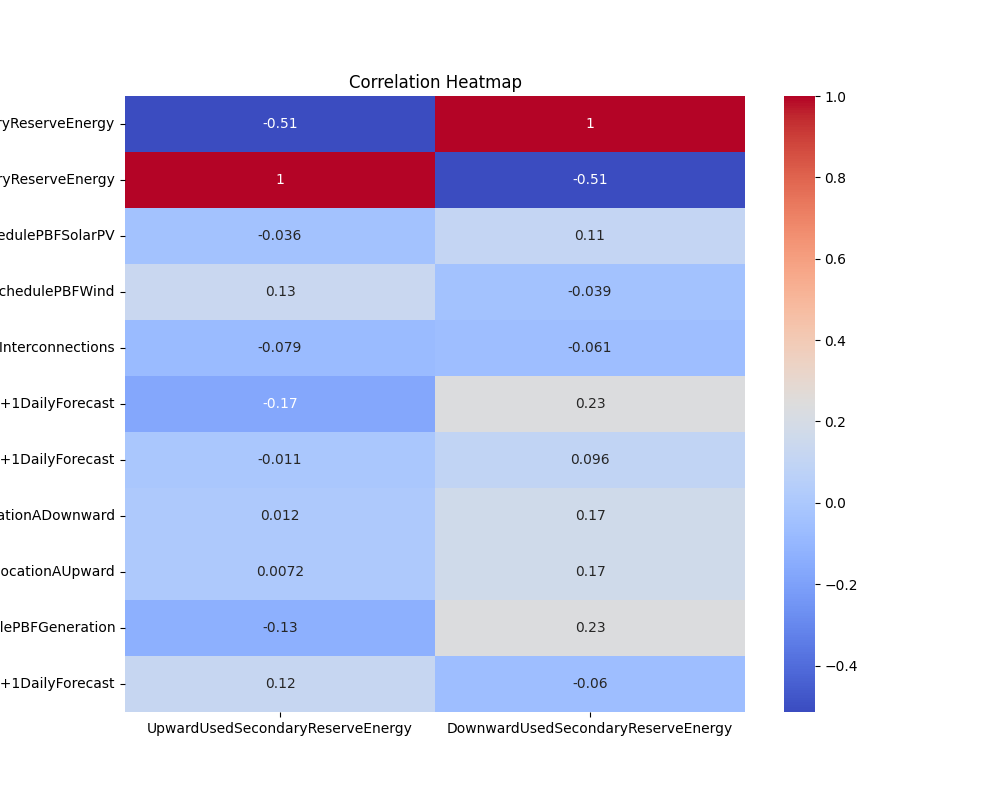
\includegraphics[height=9cm, keepaspectratio=true]{plots/correlation_heatmap.png}
    \caption{Attribute correlation}
    \label{fig:Attribute_correlation}
  \end{figure}
%   \unskip
  
 In Figure~\ref{fig:Attribute_correlation} is possible to verify that the correlation between allocated capacities and used energy is close to zero.  
  
The goal of this work is to reduce the difference between allocated capacities and used energy to efficiently use the available resources.

\subsubsection{Validation Data}
As for validation it was chosen the year 2024, with summary presented in Table~\ref{validation_data_mean}.\par
\begin{table}[H] 
    \caption{This is a table caption. Tables should be placed in the main text near to the first time they are~cited.\label{tab1}}
    \newcolumntype{C}{>{\centering\arraybackslash}X}
    \begin{tabularx}{\textwidth}{CCCCC}
    \toprule
    & \textbf{mean}	& \textbf{std}	& \textbf{min} & \textbf{max}\\
    \midrule
    Down Used & 199.69 & 212.06 & 0.00 & 1721.40 \\
    Up Allocated & 623.68 & 152.39 & 419.00 & 958.00 \\
    Down Allocated & 542.59 & 126.09 & 363.00 & 946.00 \\
    Up Used & 137.36 & 170.86 & 0.00 & 1654.80 \\
    DA Wind & 6367.23 & 3603.95 & 348.00 & 20879.30 \\
    DA PV & 2056.20 & 2889.09 & 0.00 & 11892.00 \\
    DA Demand & 27604.37 & 4476.32 & 14170.00 & 41773.00 \\
    DA Schedule Generation & 27378.12 & 4738.10 & 14394.40 & 42064.50 \\
    DA Schedule PV Generation & 2084.45 & 2905.35 & 0.00 & 12175.50 \\
    DA Schedule Wind Generation & 7091.18 & 3719.91 & 392.80 & 21330.80 \\
    DA Scheduled Tie Lines & -151.89 & 2339.57 & -7112.50 & 6769.50 \\
    \bottomrule
    \end{tabularx}
    % \noindent{\footnotesize{\textsuperscript{1} Tables may have a footer.}}
\end{table}
Using the non comparative metrics the results are presented in Table~\ref{validation_res}.

\begin{table}[H] 
    \caption{This is a table caption. Tables should be placed in the main text near to the first time they are~cited.\label{tab1}}
    \newcolumntype{C}{>{\centering\arraybackslash}X}
    \begin{tabularx}{\textwidth}{CCCCC}
    \toprule
    & \textbf{RMSE}	& \textbf{SAE}	& \textbf{AllocF} & \textbf{AllocD}\\
    \midrule
    Up Allocation (MW) & 536.55 & 17357826.75 & 152679.00 & 17205147.75 \\
    Down Allocation (MW) & 408.99 & 12981575.55 & 479191.60 & 12502383.95 \\
        \bottomrule
    \end{tabularx}
    % \noindent{\footnotesize{\textsuperscript{1} Tables may have a footer.}}
\end{table}



Table~\ref{validation_res} presents the main problems of the actual capacity allocation methodology, resulting with high: i) errors (RMSE and SAE) with used energy, ii) missing energy (AllocM), and iii) extra energy (AllocS).

The correlation between allocated energy in the current method to the used energy can be seen in Figure~\ref{fig:Attribute_correlation_benchmark}.

\begin{figure}[H]
    \centering
    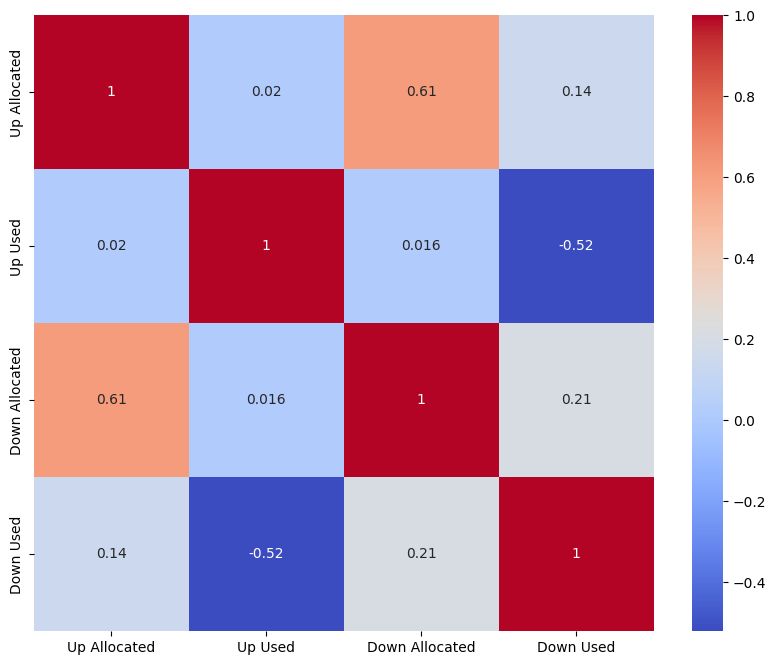
\includegraphics[width=0.75\textwidth]{plots/correlation_heatmap_benchmark.png}
    \caption{Attribute correlation benchmark}
    \label{fig:Attribute_correlation_benchmark}
  \end{figure}
%   \unskip

In Figure~\ref{fig:Attribute_correlation_benchmark} can be verified a high correlation between up and down allocated capacities, identifying the practically symmetrical used allocation.
%
Furthermore, the correlation of allocated capacities with used energy is small, which can be solved by using dynamic allocation as presented in the next section.

\subsection{Results}

The best results, only based on PPG Positive, for each architecture are presented in Tables~\ref{res_linear_forecast} and \ref{res_comparative_forecast}, were Vanilla means it is only one layer deep, and Stacked means two layers deep:

\begin{tabular}{llrrrrrrrrr}
\toprule
 &  & RMSE & SAE & AllocF & AllocD & GPD & GPD F & GPD D & GPD norm & GPD Positivo \\
 & Arquitetura &  &  &  &  &  &  &  &  &  \\
\midrule
\multirow[t]{5}{*}{Alocação a Subir} & UNET200 & 317.86 & 9759154.87 & 151181.25 & 9607973.62 & 43.78 & 0.98 & 44.16 & 22.57 & 43.78 \\
 & VanillaCNN200 & 328.88 & 10208138.49 & 147549.10 & 10060589.40 & 41.19 & 3.36 & 41.53 & 22.44 & 41.19 \\
 & UNET & 349.91 & 11008787.25 & 146742.39 & 10862044.86 & 36.58 & 3.89 & 36.87 & 20.38 & 36.58 \\
 & VanillaCNN & 370.73 & 11804382.23 & 149719.91 & 11654662.32 & 31.99 & 1.94 & 32.26 & 17.10 & 31.99 \\
 & 2StackedCNN200 & 410.28 & 13223932.55 & 126341.23 & 13097591.32 & 23.82 & 17.25 & 23.87 & 20.56 & 23.82 \\
\cline{1-11}
\multirow[t]{5}{*}{Alocação a Descer} & UNET200 & 282.52 & 8243468.87 & 469060.52 & 7774408.35 & 36.50 & 2.11 & 37.82 & 19.97 & 36.50 \\
 & VanillaCNN200 & 289.59 & 8671975.58 & 476040.73 & 8195934.85 & 33.20 & 0.66 & 34.45 & 17.55 & 33.20 \\
 & UNET & 304.28 & 9172373.23 & 470149.87 & 8702223.36 & 29.34 & 1.89 & 30.40 & 16.14 & 29.34 \\
 & VanillaCNN & 313.42 & 9483287.93 & 475881.60 & 9007406.33 & 26.95 & 0.69 & 27.95 & 14.32 & 26.95 \\
 & VanillaFCNN200 & 344.05 & 10438899.42 & 476740.17 & 9962159.25 & 19.59 & 0.51 & 20.32 & 10.41 & 19.59 \\
\cline{1-11}
\bottomrule
\end{tabular}


To choose the best model there was some analysis on \gls{PPG} and the individuals \gls{PPGS} and \gls{PPGM}. So that the final results would not just be the one best across the validation time, but also meanwise in the same time.\par
Regarding all variables in Table~\ref{training_vars}, the chosen model can be described as presented in Table~\ref{chosen_models}.
\begin{table}[H] 
    \caption{Best Model Variable Description \label{chosen_models}}
    \newcolumntype{C}{>{\centering\arraybackslash}X}
    \begin{tabularx}{\textwidth}{CCCCCC}
    \toprule
    & \textbf{Architecture}	& \textbf{Advance Loss function ratio} & \textbf{Loss function} & \textbf{Activation} & \textbf{Weights}\\
    \midrule
    Up Allocation & StackedFCNN & 0.23 & MSE & ReLU & Mean \\
    Down Allocation & StackedFCNN & 0.002 & MSE & ReLU & Mean \\
        \bottomrule
    \end{tabularx}
    % \noindent{\footnotesize{\textsuperscript{1} Tables may have a footer.}}
\end{table}

Within the validation time, best model results can be summarized by Tables~\ref{pred_res_linear} and \ref{pred_res}.

\begin{table}[H] 
    \caption{Model Metric Results for Predictions. \label{pred_res_linear}}
    \newcolumntype{C}{>{\centering\arraybackslash}X}
    \begin{tabularx}{\textwidth}{CCCCC}
    \toprule
    & \textbf{RMSE}	& \textbf{SAE}	& \textbf{AllocM} & \textbf{AllocS}\\
    \midrule
    Up Allocation (MW) & 570.21 & 4506080.04 & 40569.85 & 4465510.18 \\
    Down Allocation (MW) & 694.80 & 5811536.58 & 13619.08 & 5797917.50 \\
        \bottomrule
    \end{tabularx}
    % \noindent{\footnotesize{\textsuperscript{1} Tables may have a footer.}}
\end{table}


\begin{table}[H] 
    \caption{Model/Benchmark Comparative Metrics Results for predictions. \label{pred_res}}
    \newcolumntype{C}{>{\centering\arraybackslash}X}
    \begin{tabularx}{\textwidth}{CCCCC}
    \toprule
    & \textbf{PPG}	& \textbf{PPG M}	& \textbf{PPG S} \\
    \midrule
    Up Allocation (\%) & 21.77 & 1.24 & 21.92 \\
    Down Allocation (\%) & 11.39 & 9.31 & 11.39 \\
        \bottomrule
    \end{tabularx}
    % \noindent{\footnotesize{\textsuperscript{1} Tables may have a footer.}}
\end{table}



When comparing Table~\ref{validation_res} with Table~\ref{pred_res_linear} can be verified a significant improvement in all outputs, supported by the metrics presented in Table~\ref{pred_res}.
%
Indeed, by using the best machine learning methodology, in Table~\ref{pred_res} is possible to verify a reduction of 21.92\% and 11.39\% in the extra up and down allocated capacity (PPG S) concerning the benchmark, respectively.
%
Furthermore, the missing allocated up and down capacity (PPG M) also reduced by 1.24\% and 9.31\% concerning the benchmark, respectively.

Table~\ref{model_vs_bench} presents the overall description and comparison of the presented model with the benchmark.
% meter tableas dos resutlados com benchmark
\begin{table}[H] 
    \caption{Model Results and (allocated) values wthin 2024.\label{model_vs_bench}}
    \begin{adjustwidth}{-\extralength}{0cm}
    \newcolumntype{C}{>{\centering\arraybackslash}X}
    \begin{tabularx}{\fulllength}{CCCCCC}
    \toprule
    & & \textbf{mean}	& \textbf{std}	& \textbf{min} & \textbf{max}\\


    \midrule
            \multirow[m]{2}{*}{Down Allocation (MW)}	        & & (921.84) & (191.03) & (720.00) & (1708.00) \\
                                                                & & 836.85 & 182.04 & 247.82 & 1469.62 \\
            \multirow[m]{2}{*}{Up Allocation (MW)}	            & & (921.49) & (191.72) & (719.00) & (1694.00) \\
                                                                & & 778.42 & 228.85 & -29.47 & 1458.01 \\
            \multirow[m]{2}{*}{Hourly Capacity (MW)}	        & & (1843.32) & (382.35) & (1439.00) & (3399.00) \\
                                                                & & 1615.27 & 346.50 & 393.85 & 2594.85 \\
            \multirow[m]{2}{*}{Extraordinary Down Energy (MWh)}	& & (168.74) & (175.69) & (0.90) & (1214.00) \\
                                                                & & 149.66 & 179.96 & 2.66 & 1358.81 \\   
            \multirow[m]{2}{*}{Extraordinary Up Energy (MWh)}	& & (179.39) & (163.94) & (1.00) & (1054.80) \\
                                                                & & 141.85 & 153.57 & 1.83 & 1420.22 \\
    \bottomrule
    \end{tabularx}
    \end{adjustwidth}
\end{table}


The proposed model presents an overall improvement of \textasciitilde22\% in upward allocation and \textasciitilde11\% in downward allocation, comparing to current allocation methods.\par
Where the hourly means differences between benchmark and validation results are presented in Table~\ref{model_vs_bench_perc}.

% meter tableas dos resutlados dos deltas com benchmark
\begin{table}[H] 
    \caption{Mean $\Delta$\% between model and benchmark\label{model_vs_bench_perc}}
    \newcolumntype{C}{>{\centering\arraybackslash}X}
    \begin{tabularx}{\textwidth}{CC}
    \toprule
    & \textbf{$\Delta$\%} \\
    

    \midrule
            Down Allocation (MW)	        & -28.62 \\
            Up Allocation (MW)              & -37.26 \\
            Hourly Capacity (MW)	        & -33.24 \\
            Extraordinary Down Energy (MWh)	& -51.62 \\
            Extraordinary Up Energy (MWh)	& -59.47 \\
    \bottomrule
    \end{tabularx}
    % \noindent{\footnotesize{\textsuperscript{1} Tables may have a footer.}}
\end{table}




Average hourly improvements are of \textasciitilde16\% and \textasciitilde9\% respectively, which also is an improvement on state of the art \cite{Algarvio2024} with 13\% and 8\%.
The current study can free in average \textasciitilde12\% of hourly resources, lowering the need to allocate down and up capacity to the secondary reserve in \textasciitilde21\% and \textasciitilde11\%, respectively.\par

Can also be checked that the correlation between used and alocated is bigger than in the current method, achieving 36\% in both upward energy and downward energy. \par

\begin{figure}[H]
    \centering
    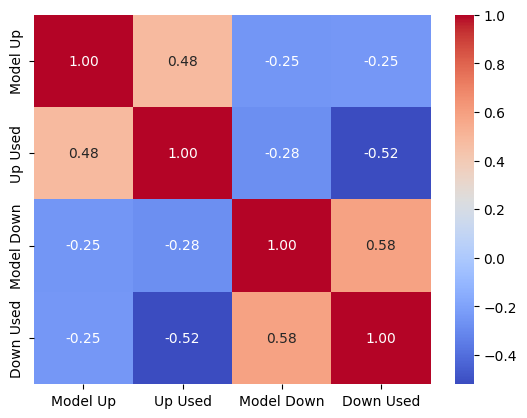
\includegraphics[width=0.75\textwidth]{plots/heatmap_correlation_pred.png}
    \caption{Attribute correlation}
    \label{fig:Attribute_correlation}
  \end{figure}


 \par

% The proposed dynamic reserve procurement methodology is implemented in three main steps:

% \subsubsection*{Forecasting Reserve Needs}
% Machine learning models are trained to predict the upward and downward reserve requirements based on day-ahead forecasts of vRES generation and system demand. Models such as Long Short-Term Memory (LSTM) networks, Random Forests, and XGBoost are used to capture temporal and nonlinear dependencies in the data. The inputs to the models include historical forecasts, real-time deviations, and weather data.

% \subsubsection*{Dynamic Allocation of Reserves}
% Using the machine learning forecasts, the required reserve capacities are dynamically adjusted for upward and downward reserves. The allocation considers real-time deviations observed in previous periods and adjusts procurement to better match actual system needs.

% \subsubsection*{Performance Evaluation}
% The performance of the dynamic reserve procurement is evaluated using key metrics, including:
% \begin{itemize}
%     \item \textbf{Forecast Error (RMSE and MAE)}: Measures the accuracy of reserve predictions.
%     \item \textbf{Reserve Utilization Rate}: Assesses the alignment between procured and activated reserves.
%     \item \textbf{Cost Efficiency}: Compares the costs of dynamic procurement with traditional static methods.
% \end{itemize}

% \subsection*{Results and Analysis}
% The results of the case study demonstrate significant improvements in reserve allocation efficiency compared to the traditional static methods currently used by the Spanish TSO.

% \subsubsection*{Forecast Accuracy}
% The machine learning models, particularly the LSTM network, outperformed traditional statistical methods such as ARIMA in predicting reserve requirements. The Root Mean Square Error (RMSE) was reduced by 15-20\% for both upward and downward reserve predictions.

% Incorporating weather variables into the models significantly improved the accuracy of vRES generation forecasts, which directly influenced reserve predictions.

% \subsubsection*{Reserve Utilization}
% The dynamic approach led to a higher utilization rate of procured reserves. The proportion of unused reserves was reduced by approximately 10\%, indicating a better alignment between forecasted and actual reserve needs.

% Asymmetrical reserve procurement allowed for flexibility in addressing specific system needs, such as prioritizing downward reserves during periods of high solar generation.

% \subsubsection*{Cost Efficiency}
% The dynamic procurement methodology reduced total reserve procurement costs by 8-12\% compared to static allocation methods. This cost savings was primarily driven by the reduction in over-procurement of reserves.

% The analysis showed that the optimized reserve allocation minimized the activation of expensive balancing reserves in the real-time market, further improving cost efficiency.

% \subsubsection*{Impact of vRES Penetration}
% The benefits of dynamic procurement were more pronounced during periods of high vRES penetration, where forecast uncertainty and variability were greatest. This highlights the importance of adapting reserve allocation methodologies to accommodate the increasing share of renewable generation.

\label{case_study}

\section{Conclusions}
The results of the case study validate the effectiveness of machine learning techniques in improving the accuracy of reserve forecasts and optimizing reserve allocation. By dynamically adjusting upward and downward reserves based on real-time forecasts, the proposed methodology addresses the inefficiencies of static procurement methods. The observed cost savings and improved reserve utilization demonstrate the practical benefits of this approach for systems with high renewable penetration.

Additionally, the case study highlights the potential for asymmetrical dynamic reserve procurement to better reflect system needs, particularly during periods of extreme renewable generation variability. The integration of weather forecasts into the predictive models further enhances their reliability, ensuring that reserve procurement decisions are informed by real-time conditions.

Using the StackedFCNN architecture the average hourly improvements are of \textasciitilde16\% and \textasciitilde9\%, respectively.
By using this leaning architecture the average hourly secondary allocated capacity can be reduced by \textasciitilde12\%, lowering the hourly need to allocate down and up capacities in \textasciitilde11\% and \textasciitilde21\%, respectively.

In conclusion, the case study illustrates that dynamic reserve procurement, supported by machine learning techniques, can significantly improve the efficiency and cost-effectiveness of balancing services in modern electricity systems. These findings provide a strong foundation for further research and potential implementation in other balancing markets with similar challenges.

For future work, a daily operational machine learning methodology will be developed, considering daily training data updates to better correlate reserved capacity with real-time reserve needs.

\authorcontributions{{Conceptualization, J.S and H.A.; Methodology, J.S and H.A.; Software, J.S.; Validation, H.A.; Formal analysis, J.S and H.A.; Investigation, J.S and H.A.; Resources, J.S and H.A.; Data curation, J.S and H.A.; Writing---original draft, J.S.; Writing---review \& editing, H.A; Visualization, J.S.; Supervision, H.A.; Project administration, H.A.; Funding acquisition, H.A. All authors have read and agreed to the published version of the manuscript.}}

\funding{This work received funding from the EU Horizon 2020 research and innovation program under the project TradeRES (grant agreement no. 864276).}

%\institutionalreview{Not applicable}
%
%\informedconsent{Not applicable}

\supplementary{All methodologies are provided to allow the replicability of this work and testing them on other markets. IterativeImputer data preprocessing methodology is at \url{https://scikit-learn.org/stable/modules/generated/sklearn.impute.IterativeImputer.html}. Alquimodelia model can be obtained at \url{https://github.com/alquimodelia}. Mirror Weights ratio methodology is at \url{https://github.com/alquimodelia/alquitable/blob/main/alquitable/advanced_losses.py\#L33}. Alquitable workshop package is at \url{https://github.com/alquimodelia/alquitable}. MuadDib machine learning framework can be obtained at \url{https://github.com/alquimodelia/MuadDib}.
}


\dataavailability{The data used to dynamically forecast secondary reserve needs and validate the proposed model is available at \url{https://www.esios.ree.es/es}.
}
%%%%%%%%%%%%%%%%%%%%%%%%%%%%%%%%%%%%%%%%%%
%\acknowledgments{In this section, you can acknowledge any support given which is not covered by the author contribution or funding sections. This may include administrative and technical support, or donations in kind (e.g., materials used for experiments).}

%%%%%%%%%%%%%%%%%%%%%%%%%%%%%%%%%%%%%%%%%%
\conflictsofinterest{The authors declare no conflicts of interest.} 
\label{conclusion}


%%%%%%%%%%%%%%%%%%%%%%%%%%%%%%%%%%%%%%%%%%
%%%%%%%%%%%%%%%%%%%%%%%%%%%%%%%%%%%%%%%%%%
%%%%%%%%%%%%%%%%%%%%%%%%%%%%%%%%%%%%%%%%%%




%%%%%%%%%%%%%%%%%%%%%%%%%%%%%%%%%%%%%%%%%%
% \section{Materials and Methods}

% Materials and Methods should be described with sufficient details to allow others to replicate and build on published results. Please note that publication of your manuscript implicates that you must make all materials, data, computer code, and protocols associated with the publication available to readers. Please disclose at the submission stage any restrictions on the availability of materials or information. New methods and protocols should be described in detail while well-established methods can be briefly described and appropriately cited.

% Research manuscripts reporting large datasets that are deposited in a publicly avail-able database should specify where the data have been deposited and provide the relevant accession numbers. If the accession numbers have not yet been obtained at the time of submission, please state that they will be provided during review. They must be provided prior to publication.

% Interventionary studies involving animals or humans, and other studies require ethical approval must list the authority that provided approval and the corresponding ethical approval code.
% \begin{quote}
% This is an example of a quote.
% \end{quote}

% %%%%%%%%%%%%%%%%%%%%%%%%%%%%%%%%%%%%%%%%%%
% \section{Results}

% This section may be divided by subheadings. It should provide a concise and precise description of the experimental results, their interpretation as well as the experimental conclusions that can be drawn.
% \subsection{Subsection}
% \subsubsection{Subsubsection}

% Bulleted lists look like this:
% \begin{itemize}
% \item	First bullet;
% \item	Second bullet;
% \item	Third bullet.
% \end{itemize}

% Numbered lists can be added as follows:
% \begin{enumerate}
% \item	First item; 
% \item	Second item;
% \item	Third item.
% \end{enumerate}

% The text continues here. 

% \subsection{Figures, Tables and Schemes}

% All figures and tables should be cited in the main text as Figure~\ref{fig1}, Table~\ref{tab1}, etc.

% \begin{figure}[H]
% 
\includegraphics[width=10.5 cm]{Definitions/logo-mdpi}
% \caption{This is a figure. Schemes follow the same formatting. If there are multiple panels, they should be listed as: (\textbf{a}) Description of what is contained in the first panel. (\textbf{b}) Description of what is contained in the second panel. Figures should be placed in the main text near to the first time they are cited. A caption on a single line should be centered.\label{fig1}}
% \end{figure}   
% \unskip

% \begin{table}[H] 
% \caption{This is a table caption. Tables should be placed in the main text near to the first time they are~cited.\label{tab1}}
% \newcolumntype{C}{>{\centering\arraybackslash}X}
% \begin{tabularx}{\textwidth}{CCC}
% \toprule
% \textbf{Title 1}	& \textbf{Title 2}	& \textbf{Title 3}\\
% \midrule
% Entry 1		& Data			& Data\\
% Entry 2		& Data			& Data \textsuperscript{1}\\
% \bottomrule
% \end{tabularx}
% \noindent{\footnotesize{\textsuperscript{1} Tables may have a footer.}}
% \end{table}

% The text continues here (Figure~\ref{fig2} and Table~\ref{tab2}).

% % Example of a figure that spans the whole page width. The same concept works for tables, too.
% \begin{figure}[H]
% \begin{adjustwidth}{-\extralength}{0cm}
% \centering
% 
\includegraphics[width=15.5cm]{Definitions/logo-mdpi}
% \end{adjustwidth}
% \caption{This is a wide figure.\label{fig2}}
% \end{figure}  

% \begin{table}[H]
% \caption{This is a wide table.\label{tab2}}
% 	\begin{adjustwidth}{-\extralength}{0cm}
% 		\newcolumntype{C}{>{\centering\arraybackslash}X}
% 		\begin{tabularx}{\fulllength}{CCCC}
% 			\toprule
% 			\textbf{Title 1}	& \textbf{Title 2}	& \textbf{Title 3}     & \textbf{Title 4}\\
% 			\midrule
% \multirow[m]{3}{*}{Entry 1 *}	& Data			& Data			& Data\\
% 			  	                   & Data			& Data			& Data\\
% 			             	      & Data			& Data			& Data\\
%                    \midrule
% \multirow[m]{3}{*}{Entry 2}    & Data			& Data			& Data\\
% 			  	                  & Data			& Data			& Data\\
% 			             	     & Data			& Data			& Data\\
%                    \midrule
% \multirow[m]{3}{*}{Entry 3}    & Data			& Data			& Data\\
% 			  	                 & Data			& Data			& Data\\
% 			             	    & Data			& Data			& Data\\
%                   \midrule
% \multirow[m]{3}{*}{Entry 4}   & Data			& Data			& Data\\
% 			  	                 & Data			& Data			& Data\\
% 			             	    & Data			& Data			& Data\\
% 			\bottomrule
% 		\end{tabularx}
% 	\end{adjustwidth}
% 	\noindent{\footnotesize{* Tables may have a footer.}}
% \end{table}

% %\begin{listing}[H]
% %\caption{Title of the listing}
% %\rule{\columnwidth}{1pt}
% %\raggedright Text of the listing. In font size footnotesize, small, or normalsize. Preferred format: left aligned and single spaced. Preferred border format: top border line and bottom border line.
% %\rule{\columnwidth}{1pt}
% %\end{listing}

% Text.

% Text.

% \subsection{Formatting of Mathematical Components}

% This is the example 1 of equation:
% \begin{linenomath}
% \begin{equation}
% a = 1,
% \end{equation}
% \end{linenomath}
% the text following an equation need not be a new paragraph. Please punctuate equations as regular text.
% %% If the documentclass option "submit" is chosen, please insert a blank line before and after any math environment (equation and eqnarray environments). This ensures correct linenumbering. The blank line should be removed when the documentclass option is changed to "accept" because the text following an equation should not be a new paragraph.

% This is the example 2 of equation:
% \begin{adjustwidth}{-\extralength}{0cm}
% \begin{equation}
% a = b + c + d + e + f + g + h + i + j + k + l + m + n + o + p + q + r + s + t + u + v + w + x + y + z
% \end{equation}
% \end{adjustwidth}

% % Example of a page in landscape format (with table and table footnote).
% %\startlandscape
% %\begin{table}[H] %% Table in wide page
% %\caption{This is a very wide table.\label{tab3}}
% %	\begin{tabularx}{\textwidth}{CCCC}
% %		\toprule
% %		\textbf{Title 1}	& \textbf{Title 2}	& \textbf{Title 3}	& \textbf{Title 4}\\
% %		\midrule
% %		Entry 1		& Data			& Data			& This cell has some longer content that runs over two lines.\\
% %		Entry 2		& Data			& Data			& Data\textsuperscript{1}\\
% %		\bottomrule
% %	\end{tabularx}
% %	\begin{adjustwidth}{+\extralength}{0cm}
% %		\noindent\footnotesize{\textsuperscript{1} This is a table footnote.}
% %	\end{adjustwidth}
% %\end{table}
% %\finishlandscape


% Please punctuate equations as regular text. Theorem-type environments (including propositions, lemmas, corollaries etc.) can be formatted as follows:
% %% Example of a theorem:
% \begin{Theorem}
% Example text of a theorem.
% \end{Theorem}

% The text continues here. Proofs must be formatted as follows:

% %% Example of a proof:
% \begin{proof}[Proof of Theorem 1]
% Text of the proof. Note that the phrase ``of Theorem 1'' is optional if it is clear which theorem is being referred to.
% \end{proof}
% The text continues here.

% %%%%%%%%%%%%%%%%%%%%%%%%%%%%%%%%%%%%%%%%%%
% \section{Discussion}

% Authors should discuss the results and how they can be interpreted from the perspective of previous studies and of the working hypotheses. The findings and their implications should be discussed in the broadest context possible. Future research directions may also be highlighted.

% %%%%%%%%%%%%%%%%%%%%%%%%%%%%%%%%%%%%%%%%%%
% \section{Conclusions}

% This section is not mandatory, but can be added to the manuscript if the discussion is unusually long or complex.

% %%%%%%%%%%%%%%%%%%%%%%%%%%%%%%%%%%%%%%%%%%
% \section{Patents}

% This section is not mandatory, but may be added if there are patents resulting from the work reported in this manuscript.

%%%%%%%%%%%%%%%%%%%%%%%%%%%%%%%%%%%%%%%%%%
\vspace{6pt} 

%%%%%%%%%%%%%%%%%%%%%%%%%%%%%%%%%%%%%%%%%%
%% optional
%\supplementary{The following supporting information can be downloaded at:  \linksupplementary{s1}, Figure S1: title; Table S1: title; Video S1: title.}

% Only for journal Methods and Protocols:
% If you wish to submit a video article, please do so with any other supplementary material.
% \supplementary{The following supporting information can be downloaded at: \linksupplementary{s1}, Figure S1: title; Table S1: title; Video S1: title. A supporting video article is available at doi: link.}

% Only for journal Hardware:
% If you wish to submit a video article, please do so with any other supplementary material.
% \supplementary{The following supporting information can be downloaded at: \linksupplementary{s1}, Figure S1: title; Table S1: title; Video S1: title.\vspace{6pt}\\
%\begin{tabularx}{\textwidth}{lll}
%\toprule
%\textbf{Name} & \textbf{Type} & \textbf{Description} \\
%\midrule
%S1 & Python script (.py) & Script of python source code used in XX \\
%S2 & Text (.txt) & Script of modelling code used to make Figure X \\
%S3 & Text (.txt) & Raw data from experiment X \\
%S4 & Video (.mp4) & Video demonstrating the hardware in use \\
%... & ... & ... \\
%\bottomrule
%\end{tabularx}
%}

%%%%%%%%%%%%%%%%%%%%%%%%%%%%%%%%%%%%%%%%%%
% \authorcontributions{For research articles with several authors, a short paragraph specifying their individual contributions must be provided. The following statements should be used ``Conceptualization, X.X. and Y.Y.; methodology, X.X.; software, X.X.; validation, X.X., Y.Y. and Z.Z.; formal analysis, X.X.; investigation, X.X.; resources, X.X.; data curation, X.X.; writing---original draft preparation, X.X.; writing---review and editing, X.X.; visualization, X.X.; supervision, X.X.; project administration, X.X.; funding acquisition, Y.Y. All authors have read and agreed to the published version of the manuscript.'', please turn to the  \href{http://img.mdpi.org/data/contributor-role-instruction.pdf}{CRediT taxonomy} for the term explanation. Authorship must be limited to those who have contributed substantially to the work~reported.}

% \funding{Please add: ``This research received no external funding'' or ``This research was funded by NAME OF FUNDER grant number XXX.'' and  and ``The APC was funded by XXX''. Check carefully that the details given are accurate and use the standard spelling of funding agency names at \url{https://search.crossref.org/funding}, any errors may affect your future funding.}

% \institutionalreview{In this section, you should add the Institutional Review Board Statement and approval number, if relevant to your study. You might choose to exclude this statement if the study did not require ethical approval. Please note that the Editorial Office might ask you for further information. Please add “The study was conducted in accordance with the Declaration of Helsinki, and approved by the Institutional Review Board (or Ethics Committee) of NAME OF INSTITUTE (protocol code XXX and date of approval).” for studies involving humans. OR “The animal study protocol was approved by the Institutional Review Board (or Ethics Committee) of NAME OF INSTITUTE (protocol code XXX and date of approval).” for studies involving animals. OR “Ethical review and approval were waived for this study due to REASON (please provide a detailed justification).” OR “Not applicable” for studies not involving humans or animals.}

% \informedconsent{Any research article describing a study involving humans should contain this statement. Please add ``Informed consent was obtained from all subjects involved in the study.'' OR ``Patient consent was waived due to REASON (please provide a detailed justification).'' OR ``Not applicable'' for studies not involving humans. You might also choose to exclude this statement if the study did not involve humans.

% Written informed consent for publication must be obtained from participating patients who can be identified (including by the patients themselves). Please state ``Written informed consent has been obtained from the patient(s) to publish this paper'' if applicable.}

% \dataavailability{We encourage all authors of articles published in MDPI journals to share their research data. In this section, please provide details regarding where data supporting reported results can be found, including links to publicly archived datasets analyzed or generated during the study. Where no new data were created, or where data is unavailable due to privacy or ethical restrictions, a statement is still required. Suggested Data Availability Statements are available in section ``MDPI Research Data Policies'' at \url{https://www.mdpi.com/ethics}.} 

% % Only for journal Nursing Reports
% %\publicinvolvement{Please describe how the public (patients, consumers, carers) were involved in the research. Consider reporting against the GRIPP2 (Guidance for Reporting Involvement of Patients and the Public) checklist. If the public were not involved in any aspect of the research add: ``No public involvement in any aspect of this research''.}

% % Only for journal Nursing Reports
% %\guidelinesstandards{Please add a statement indicating which reporting guideline was used when drafting the report. For example, ``This manuscript was drafted against the XXX (the full name of reporting guidelines and citation) for XXX (type of research) research''. A complete list of reporting guidelines can be accessed via the equator network: \url{https://www.equator-network.org/}.}

% % Only for journal Nursing Reports
% %\useofartificialintelligence{Please describe in detail any and all uses of artificial intelligence (AI) or AI-assisted tools used in the preparation of the manuscript. This may include, but is not limited to, language translation, language editing and grammar, or generating text. Alternatively, please state that “AI or AI-assisted tools were not used in drafting any aspect of this manuscript”.}

% \acknowledgments{In this section you can acknowledge any support given which is not covered by the author contribution or funding sections. This may include administrative and technical support, or donations in kind (e.g., materials used for experiments).}

% \conflictsofinterest{Declare conflicts of interest or state ``The authors declare no conflicts of interest.'' Authors must identify and declare any personal circumstances or interest that may be perceived as inappropriately influencing the representation or interpretation of reported research results. Any role of the funders in the design of the study; in the collection, analyses or interpretation of data; in the writing of the manuscript; or in the decision to publish the results must be declared in this section. If there is no role, please state ``The funders had no role in the design of the study; in the collection, analyses, or interpretation of data; in the writing of the manuscript; or in the decision to publish the results''.} 

%%%%%%%%%%%%%%%%%%%%%%%%%%%%%%%%%%%%%%%%%%
%% Optional

%% Only for journal Encyclopedia
%\entrylink{The Link to this entry published on the encyclopedia platform.}

% \abbreviations{Abbreviations}{
% The following abbreviations are used in this manuscript:\\

% \noindent 
% \begin{tabular}{@{}ll}
% MDPI & Multidisciplinary Digital Publishing Institute\\
% DOAJ & Directory of open access journals\\
% TLA & Three letter acronym\\
% LD & Linear dichroism
% \end{tabular}
% }

\abbreviations{Abbreviations}{
The following abbreviations are used in this manuscript:\\

\noindent 
	
	\printglossary[type=\acronymtype, style=long]
}

%%%%%%%%%%%%%%%%%%%%%%%%%%%%%%%%%%%%%%%%%%
%% Optional
\appendixtitles{no} % Leave argument "no" if all appendix headings stay EMPTY (then no dot is printed after "Appendix A"). If the appendix sections contain a heading then change the argument to "yes".
\appendixstart
\appendix
\section[\appendixname~\thesection]{}
\subsection[\appendixname~\thesubsection]{}
The appendix is an optional section that can contain details and data supplemental to the main text---for example, explanations of experimental details that would disrupt the flow of the main text but nonetheless remain crucial to understanding and reproducing the research shown; figures of replicates for experiments of which representative data are shown in the main text can be added here if brief, or as Supplementary Data. Mathematical proofs of results not central to the paper can be added as an appendix.

\begin{table}[H] 
\caption{This is a table caption.\label{tab5}}
\newcolumntype{C}{>{\centering\arraybackslash}X}
\begin{tabularx}{\textwidth}{CCC}
\toprule
\textbf{Title 1}	& \textbf{Title 2}	& \textbf{Title 3}\\
\midrule
Entry 1		& Data			& Data\\
Entry 2		& Data			& Data\\
\bottomrule
\end{tabularx}
\end{table}

\section[\appendixname~\thesection]{}
All appendix sections must be cited in the main text. In the appendices, Figures, Tables, etc. should be labeled, starting with ``A''---e.g., Figure A1, Figure A2, etc.

%%%%%%%%%%%%%%%%%%%%%%%%%%%%%%%%%%%%%%%%%%
\begin{adjustwidth}{-\extralength}{0cm}
%\printendnotes[custom] % Un-comment to print a list of endnotes

\reftitle{References}

% Please provide either the correct journal abbreviation (e.g. according to the “List of Title Word Abbreviations” http://www.issn.org/services/online-services/access-to-the-ltwa/) or the full name of the journal.
% Citations and References in Supplementary files are permitted provided that they also appear in the reference list here. 

%=====================================
% References, variant A: external bibliography
%=====================================
\bibliography{export, ../../dissertation/library}

%=====================================
% References, variant B: internal bibliography
%=====================================
% \begin{thebibliography}{999}
% % Reference 1
% \bibitem[Author1(year)]{ref-journal}
% Author~1, T. The title of the cited article. {\em Journal Abbreviation} {\bf 2008}, {\em 10}, 142--149.
% % Reference 2
% \bibitem[Author2(year)]{ref-book1}
% Author~2, L. The title of the cited contribution. In {\em The Book Title}; Editor 1, F., Editor 2, A., Eds.; Publishing House: City, Country, 2007; pp. 32--58.
% % Reference 3
% \bibitem[Author3(year)]{ref-book2}
% Author 1, A.; Author 2, B. \textit{Book Title}, 3rd ed.; Publisher: Publisher Location, Country, 2008; pp. 154--196.
% % Reference 4
% \bibitem[Author4(year)]{ref-unpublish}
% Author 1, A.B.; Author 2, C. Title of Unpublished Work. \textit{Abbreviated Journal Name} year, \textit{phrase indicating stage of publication (submitted; accepted; in press)}.
% % Reference 5
% \bibitem[Author5(year)]{ref-communication}
% Author 1, A.B. (University, City, State, Country); Author 2, C. (Institute, City, State, Country). Personal communication, 2012.
% % Reference 6
% \bibitem[Author6(year)]{ref-proceeding}
% Author 1, A.B.; Author 2, C.D.; Author 3, E.F. Title of presentation. In Proceedings of the Name of the Conference, Location of Conference, Country, Date of Conference (Day Month Year); Abstract Number (optional), Pagination (optional).
% % Reference 7
% \bibitem[Author7(year)]{ref-thesis}
% Author 1, A.B. Title of Thesis. Level of Thesis, Degree-Granting University, Location of University, Date of Completion.
% % Reference 8
% \bibitem[Author8(year)]{ref-url}
% Title of Site. Available online: URL (accessed on Day Month Year).
% \end{thebibliography}

% If authors have biography, please use the format below
%\section*{Short Biography of Authors}
%\bio
%{\raisebox{-0.35cm}{\includegraphics[width=3.5cm,height=5.3cm,clip,keepaspectratio]{Definitions/author1.pdf}}}
%{\textbf{Firstname Lastname} Biography of first author}
%
%\bio
%{\raisebox{-0.35cm}{\includegraphics[width=3.5cm,height=5.3cm,clip,keepaspectratio]{Definitions/author2.jpg}}}
%{\textbf{Firstname Lastname} Biography of second author}

% For the MDPI journals use author-date citation, please follow the formatting guidelines on http://www.mdpi.com/authors/references
% To cite two works by the same author: \citeauthor{ref-journal-1a} (\citeyear{ref-journal-1a}, \citeyear{ref-journal-1b}). This produces: Whittaker (1967, 1975)
% To cite two works by the same author with specific pages: \citeauthor{ref-journal-3a} (\citeyear{ref-journal-3a}, p. 328; \citeyear{ref-journal-3b}, p.475). This produces: Wong (1999, p. 328; 2000, p. 475)

%%%%%%%%%%%%%%%%%%%%%%%%%%%%%%%%%%%%%%%%%%
%% for journal Sci
%\reviewreports{\\
%Reviewer 1 comments and authors’ response\\
%Reviewer 2 comments and authors’ response\\
%Reviewer 3 comments and authors’ response
%}
%%%%%%%%%%%%%%%%%%%%%%%%%%%%%%%%%%%%%%%%%%
\PublishersNote{}
\end{adjustwidth}
\end{document}

